\chapter{Real Analysis: Divergence Theorem \& Measure Theory}

\section{Recall: The Divergence Theorem}

\begin{spoken-clean}[00:00:00 - 00:02:19]
I brought back the \qt{gavel} because today I expect an \qt{extra circus}. Remember that I told you the first day, the final goal, or the \qt{final boss} of Analysis II, or one of the most representative theorems, is this Divergence Theorem. On the first day, I needed to state it very informally, using \qt{potatoes} and stuff, because you didn't know any of the mathematical elements. But now, we saw the statement again some weeks ago, and we already knew some parts. And now we know almost all of it.

Let me remind you of the statement. We know many elements now. $\Omega$ in $\mathbb{R}^n$ is an open, bounded set. Its boundary, $\partial\Omega$, will be a $C^1$ submanifold. This we know what it means. $F$ will be a $C^1$ function up to the boundary, taking values in $\mathbb{R}^n$. This is a vector field. You can imagine this function as a vector field. And the theorem says that the integral over $\Omega$ of this combination of partial derivatives (i.e., the partial derivative with respect to $x_i$ of the $i$-th component of the vector field, summed over $i$) integrated with respect to the Jordan measure (i.e., the Riemann integral) is equal to this integral over the boundary of the domain with respect to the surface measure of the boundary. We know that $F \cdot \nu$ is $F$ multiplied by the normal vector, which we already saw what a tangent vector and a normal vector to the boundary are. So, more or less everything you know what it is now, except for one thing. This (i.e., the integral over the boundary) goes with this (i.e., the surface measure $dS$). The integral over a surface of the differential of volume in the surface. We know how to integrate on the full space, but not over a curved surface. And this is where we are going today. We are going to learn, we are going to define what is the integral over the surface.
\end{spoken-clean}

\begin{math-stroke}[The Divergence Theorem]
\begin{nice-box}[Divergence Theorem]
\begin{theorem}[Divergence Theorem]
Let $\Omega \subset \mathbb{R}^n$ be an open, bounded set, and let $\partial\Omega$ be a $C^1$ submanifold.
Let $F \in C^1(\overline{\Omega}, \mathbb{R}^n)$ be a vector field. Then:
\[
\int_{\Omega} \sum_{i=1}^n \partial_i F_i \, dx = \int_{\partial\Omega} F \cdot \underbrace{\nu}_{\text{unit vector normal to } \partial\Omega} \, \underbrace{dS}_{\mathclap{\substack{\text{Surface measure} \\ \text{(Goal of today's lecture)}}}}
\]
\end{theorem}
\end{nice-box}
\end{math-stroke}

\section{Measuring Volumes over Submanifolds}

\begin{spoken-clean}[02:19 - 04:30]
Okay, so the next step in our quest is to define integrals over d-dimensional submanifolds. Today, we will measure volumes over submanifolds of dimension $d$. Towards this goal, we start with the easiest case. What is the easiest possible submanifold? It's the submanifold of dimension one. So, let's start by $d=1$. A submanifold of dimension one, we call it a curve. And we will see how to measure length.
\end{spoken-clean}

\begin{math-stroke}[Quest Log: From Volumes to Lengths]
The lecturer outlines the plan for the day.
\begin{description}
    \item[Next Step:] Define $\int$ over $d$-dim submanifolds.
    \item[Today's Goal:] Define how to measure volumes over submanifolds.
    \item[Starting Case:] Begin with the simplest case, $d=1$, where a submanifold is a curve and its "volume" is its length.
\end{description}
\end{math-stroke}

\begin{spoken-clean}[04:30 - 06:25]
I will work in the set of parameterized submanifolds so far, and I will give you the definition. Let me add here, over parameterized submanifolds. For today, then we will extend, but for today, let me add \emph{parameterized}. Okay.

So, a parameterized 1-manifold is a curve. Remember that we gave the definition some weeks ago. We have some $\phi$ (i.e., a map $\phi$) from $V$ to $\mathbb{R}^n$, where $V \subset \mathbb{R}$ is open. That is the parametrization. And this has to satisfy some conditions. The most important was that it is injective, and also that the differential (which in this case is just the velocity vector, $\phi'(t)$) is injective. In the case of curves, it means that this number, the velocity vector, is never zero.
\end{spoken-clean}

\begin{math-stroke}[Definition: Parameterized 1-Manifold (Curve)]
A \textbf{parameterized 1-manifold}, or curve, is defined by a map $\phi: V \to \mathbb{R}^n$, where $V \subset \mathbb{R}$ is an open set. The map must satisfy several conditions:
\begin{itemize}
    \item It must be \textbf{injective}.
    \item Its derivative must never be zero: $\phi'(t) \neq 0$.
    \item It must satisfy a topological property to prevent self-intersections where the curve loops back on itself, which is a more advanced condition from differential geometry.
\end{itemize}
\end{math-stroke}

\begin{spoken-clean}[06:25 - 08:38]
And now we will give the definition of length. So, if in this setup, if $[a,b]$ is a closed interval contained in the domain of the parametrization, then I define the length of $\phi([a,b])$ as the integral between $a$ and $b$ of the speed. This is the velocity vector, I take the modulus, and then I integrate with respect to $t$. This is the definition of length.

So let me do maybe a bit of a picture of what this situation is. So we have our $V$ here. So this will be $\mathbb{R}$, and we have our $V$. It could be an open interval or some open set. And then we have our map, that is $\phi$. And then there is the $\phi(V)$, that is some curve. And then we are taking a subset that is a closed subset here, that is $[a,b]$. And this piece is defining a closed piece of the curve. And then we are saying that by definition, the length of this red piece is this integral over there. Now I ask you, is this definition sound?
\end{spoken-clean}

\begin{math-stroke}[Definition of Arc Length]
\begin{definition}[Length of a Curve]
If $[a,b] \subset V$ is a closed interval within the domain of the parametrization $\phi$, the length of the curve segment $\phi([a,b])$ is defined as:
\[
L(\phi([a,b])) = \int_a^b |\phi'(t)| \, dt
\]
\end{definition}
\begin{center}
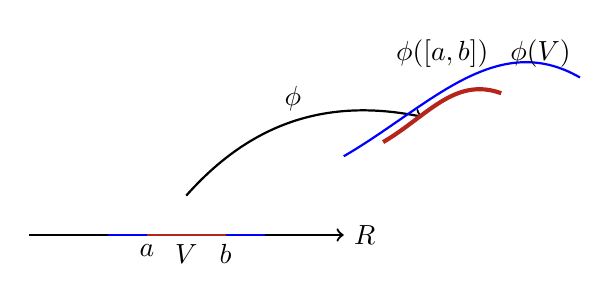
\begin{tikzpicture}
    % Domain V in R
    \draw[->, thick] (-1,0) -- (3,0) node[right] {$\mathbb{R}$};
    \draw[thick, blue] (0,0) -- (2,0);
    \node[below] at (1,0) {$V$};
    \draw[thick, BrickRed] (0.5,0) -- (1.5,0);
    \node[below] at (0.5,0) {$a$};
    \node[below] at (1.5,0) {$b$};

    % Mapping phi
    \draw[->, thick] (1, 0.5) to[bend left] node[midway, above] {$\phi$} (4, 1.5);

    % Image curve in R^n
    \draw[thick, blue] (3,1) to[out=30, in=150] (6,2);
    \node[above] at (5.5, 2) {$\phi(V)$};
    \draw[thick, BrickRed, line width=1.5pt] (3.5, 1.18) to[out=30, in=160] (5, 1.8);
    \node[above] at (4.25, 2) {$\phi([a,b])$};
\end{tikzpicture}
\end{center}
\end{math-stroke}

\begin{spoken-clean}[08:38 - 11:46]
What properties must length satisfy? And there will be four. But maybe you can tell me two, and I will complete the other two. So what should I check to see that this definition is sound? Two properties. So think that I'm defining the length of a curve, like this wire over here. What I'm saying is that to define the length of the curve, I am choosing a parametrization of the curve, I am running the curve through some map, and then I'm defining the length as this integral. Is this sound? Is this correct? What would you like to ask this definition to satisfy so that it is correct?
\end{spoken-clean}

\begin{student-question}[Student Answer]
Well, I think it should be positive, first of all. I wouldn't want to have a negative length or something like that. And I mean, this obviously satisfies that.
\end{student-question}

\begin{spoken-clean}[10:20 - 10:22]
It's positive. Okay.
\end{spoken-clean}

\begin{student-question}[Student Answer]
I also think it should be independent of $\phi$, because it should depend only on the object you measure, not on how we measure it, so to say.
\end{student-question}

\begin{spoken-clean}[10:22 - 10:23]
Louder.
\end{spoken-clean}

\begin{student-question}[Student Answer]
You should, like, the length should have additivity as one of its properties, meaning you could add the distance of two paths.
\end{student-question}

\begin{spoken-clean}[10:23 - 11:46]
So, additivity. Like the measure, right? Yes, additivity. Anything that is measuring something, if you... So additivity means that if I cut into this curve, the length of this piece plus the length of this piece is the length of the total curve. If this is not happening, the definition of length must be ill-posed, right? So we need to check that. But the additivity, since it is given by an integral, is usually very easy, right? Because integrals are additive. Okay. Some other property? I asked two, so you already did your work, but do you want to say some other property? There.
\end{spoken-clean}

\begin{student-question}[Student Answer]
It would be nice if if we have like the curve just in $\mathbb{R}$, if then it corresponds to just what we would intuitively guess.
\end{student-question}

\begin{spoken-clean}[11:46 - 13:55]
Yeah. So we can call it normalization. So he's saying that if the curve is in $\mathbb{R}$, meaning like, I guess if the curve is for instance $[0,1] \times \{0\}$, right? And this is the zero of $\mathbb{R}^{n-1}$. So the curve is just a straight segment along the $x_1$ axis, then the length of this curve should be one, right? Okay. And the last one, I will give you a hint. My curve is put in the space in some position, but this is a rigid curve, that's why I made it of thick wire. So if I put this curve in this position, or in this other position, should the length be the same? Yeah. So this is the invariance under rigid motion.
\end{spoken-clean}

\begin{math-stroke}[Axioms of Length]
For a definition of length to be sound, it must satisfy four fundamental properties:
\begin{enumerate}
    \item \textbf{Independence of Parametrization:} The length must depend only on the geometric path, not the function used to trace it.
    \item \textbf{Additivity:} If a curve is split into two segments, the total length is the sum of the segment lengths.
    \item \textbf{Invariance under Euclidean Isometry:} Rigid motions (translations and rotations) of the curve in space should not change its length.
    \item \textbf{Normalization:} The length of the standard unit interval $[0,1]$ in $\mathbb{R}$ must be 1.
\end{enumerate}
\end{math-stroke}

\begin{spoken-clean}[13:55 - 15:07]
So what is Euclidean isometry? What types of maps preserve rigid motions of the space? The rigid motions of space are translations and rotations, or compositions, right? So $F$ is a rigid motion, or a Euclidean isometry, if it is of the form $F(x) = Rx+b$, where $b$ is a vector (i.e., the translation vector) and $R$ is orthogonal. So if you want, a rotation or a symmetry or a composition of them.
\end{spoken-clean}

\begin{math-stroke}[Euclidean Isometry]
A map $F: \mathbb{R}^n \to \mathbb{R}^n$ is a \textbf{Euclidean isometry} (or rigid motion) if it has the form:
\[
F(x) = Rx+b
\]
where $R$ is an orthogonal matrix ($R^T R = I$) and $b \in \mathbb{R}^n$ is a translation vector.
\end{math-stroke}

\begin{spoken-clean}[15:07 - 17:52]
So if you take $\Psi$ from $[c,d]$ to $[a,b]$ that is bijective, $C^1$, $C^1$ inverse. Then a reparametrization is this: you would take... Let me do the drawing here. So here, you are taking some $\Psi$, and the new interval now is $[c,d]$, that maybe is longer, or maybe shorter, or maybe the speed here is irregular. Here maybe the speed is one and here the speed is irregular, right? But this map is going from here to here. Then the image of the composition of the maps is the same. So the length should be the same. And this is translated in my definition of length that I would like that when I apply this integral between $c$ and $d$ of the composition (i.e., $(\phi \circ \Psi)'(s)$) $ds$, it should be equal to the original integral (i.e., $\int_a^b |\phi'(t)| \, dt$).
This we will prove in a second, a more general property. So I think this is a good... I put this property over here as an exercise. It will follow from the more general property I will give for general $d$, right? But it's very good that you try to do this exercise by yourself. It's one line of computation if you do it right. Okay. So you need to apply the chain rule. Okay, so the additivity...
\end{spoken-clean}

\begin{math-stroke}[Invariance under Reparametrization]
Let $\Psi: [c,d] \to [a,b]$ be a bijective $C^1$ map with a $C^1$ inverse (a diffeomorphism). The reparametrized curve is $\tilde{\phi} = \phi \circ \Psi$. We must prove that $L(\tilde{\phi}) = L(\phi)$.
\[
\int_c^d |(\phi \circ \Psi)'(s)| \, ds = \int_a^b |\phi'(t)| \, dt
\]
This is left as an exercise and follows directly from the chain rule and 1D integration by substitution.
\end{math-stroke}

\begin{spoken-clean}[17:52 - 18:10]
The additivity is what I said, right? So this is property number one, property number two, the additivity is that when you have the length of $\phi([a,b])$ should be equal to the length of $\phi([a,c])$ plus the length of $\phi([c,b])$ if $c$ is any point between $a$ and $b$, for example. This is the additivity. But this follows from the additivity of the integral. So here there is nothing to prove.
\end{spoken-clean}